\documentclass[a4paper, 11pt]{article} % Font size (can be 10pt, 11pt or 12pt) and paper size (remove a4paper for US letter paper)

\usepackage[T1]{fontenc}
\usepackage[utf8]{inputenc}
\usepackage[ngerman]{babel}
\usepackage{lmodern}

\usepackage[protrusion=true,expansion=true]{microtype} % Better typography
\usepackage{graphicx} % Required for including pictures
\usepackage{wrapfig} % Allows in-line images
\usepackage{amssymb,amsmath}
\usepackage{subfigure}
\usepackage{cite}
\usepackage{mathpazo} % Use the Palatino font
\linespread{1.05} % Change line spacing here, Palatino benefits from a slight increase by default

\usepackage{tikz-uml}
%\usepackage{tikz}
%\usepackage{ifthen}
%\usepackage{xstring}
%\usepackage{calc}
%\usepackage{pgfopts}

\usepackage{listings}

%\setlength\parindent{0pt}%Festlegen des Absatzeinzuges
%\setlength\mathindent{0pt}%Festlegen des Einzuges für abgesetzte Formeln

\setlength{\parindent}{0pt} 

\makeatletter
\renewcommand\@biblabel[1]{\emph{#1.}} % Change the square brackets for each bibliography item from '[1]' to '1.'
\renewcommand{\@listI}{\itemsep=0pt} % Reduce the space between items in the itemize and enumerate environments and the bibliography

\renewcommand{\maketitle}{ % Customize the title - do not edit title and author name here, see the TITLE block below
\begin{flushright} % Right align
{\LARGE\@title} % Increase the font size of the title

\vspace{50pt} % Some vertical space between the title and author name

{\large\@author} % Author name
\\\@date % Date

\vspace{40pt} % Some vertical space between the author block and abstract
\end{flushright}
}

\title{\emph{Dokumentation gMix-Simulator GUI}\\ % Title
Benutzer- / Entwicklerhandbuch} % Subtitle

\author{\textsc{Beifuß A. ; Langnickel J. ; Lohmueller J. C. ; Weinschenk M.} % Author
\\{\textit{Universität Hamburg - MIN Falkultaet - Informatik - SVS}}} % Institution

\date{\today} % Date

\begin{document}

\maketitle % Print the title section

%\renewcommand{\abstractname}{Summary} % Uncomment to\texttt{} change the name of the abstract to something else
 
% \begin{abstract}

% \end{abstract}

\newpage
\tableofcontents

% \hspace*{3,6mm}\textit{Keywords:} lorem , ipsum , dolor , sit amet , lectus % Keywords

\vspace{30pt} % Some vertical space between the abstract and first section

\newpage
\section{Einleitung} % (fold)
\label{sec:einleitung}

\subsection{gMix} % (fold)
\label{sub:gmix}
Mixe ermöglichen die anonyme Kommunikation im Internet. Obwohl ihre Funktionsweise schon 1981 von David Chaum \cite{Cha81} beschrieben wurde, sind bisher erst wenige Dienste etabliert, die diese Technik Nutzen ( z.B. Tor \cite{DMS04} oder JAP (JonDonym) \cite{BFK01}). Allen ist gemein, dass Nachrichten der einzelnen Kommunikationspartner mit Nachrichten anderer Dienstnutzer vermischt werden, um so die Zuordnung von Nachrichten und Kommunikationsbeziehungen zu erschweren bzw. unmöglich zu machen.
\\

Dass bisher nur wenige der theoretischen Konzepte für Mixe auch in einer Implementierung umgesetzt wurden, führt zu einigen Schwierigkeiten bei der Weiterentwicklung von Mixen. Zum einen ist es schwieriger, sich mit den rein theoretischen Konzepten eingehend zu befassen, verglichen mit jenen, die bereits umgesetzt wurden und daher ausführlicher untersuchbar sind. Zum anderen müssen viele Grundkonzepte häufig neu implementiert werden oder sind noch nicht hinreichend gut verstanden, so dass Neuimplementierungen aufwendig sind. Und schließlich sind die verschiedenen bisher realisierten Mix-Techniken nur schwer vergleichbar, da sie nicht einheitlich genug umgesetzt wurden, um sie unter gleichen Bedingungen testen zu können.
\\

gMix \cite{FHF12} ist als pluginbasiertes Framework konzipiert, bei dem die Funktion verschiedener Mixe untersucht werden kann. Es werden dabei folgende Ziele angestrebt:
\begin{itemize}
\item Bereitstellung eines umfassenden Code-Repositorys mit kompatiblen und leicht erweiterbaren Mix-Implementierungen. 
\item Vereinfachen der Entwicklung neuer und praktisch nutzbarer Mixe.
\item Evaluation existierender und neuer Mix-Techniken unter einheitlichen Bedingungen.
\item Unterstützung der Lehre durch leicht zugängliche und verständliche Mix-Lösungen.
\item Motivation von Wissenschaftlern, Implementierungen auf Basis von gMix zu entwickeln und somit zu seiner Weiterentwicklung bei zu tragen.
\end{itemize}

Da grade für Pluginentwickler der Aufbau von gMix interessant sein dürfte, ist dieser Abschnitt eine zusammenfassende Übersetzung von Teilen aus ''Introducing the gMix Open Source Framework
for Mix Implementations'' von Fuchs et al. \cite{FHF12}.\\

Durch den offenen Aufbau ist es möglich, verschiedene Mixe aus den einzelnen Plugins zusammen zu stellen oder neue Plugins hinzu zu fügen. Da all diese Mixe auf die gleiche Weise erstellt werden, können sie anschließend unter den selben Bedingungen betrieben oder simuliert werden und bleiben vergleichbar.
\\

gMix ist in Layern organisiert, wie man es vom TCP/IP-Protokollstack oder dem OSI-Modell kennt und in Abbildung \ref{img:gMixLayers} dargestellt ist. Diese Layer bilden dabei zusammen einen Anonymisierungslayer, der sich in diesen Modellen zwischen Schicht 4 und 5, also zwischen der Transport- und den höheren Schichten einordnen lässt. gMix selbst hat intern 7 Layer:
\begin{itemize}
	\item Layer 6 sind die tatsächlichen Anwendungen bzw. deren Repräsentationen, also alles was sich im OSI-Modell oberhalb der Transportschicht befindet. In einer Simulation befinden sich in dieser Schicht die Lastgeneratoren und -Senken.
	\item Layer 5 stellt die Ende-Zu-Ende-Verbindungen für Prozesse her und verbirgt die Anonymisierung vor den Elementen aus Layer 6.
	\item Layer 4 realisiert die anonyme Ende-zu-Ende-Verbindung zwischen zwei Endknoten. Auf dieser Ebene werden Knoten anhand von „Global Identifieres“ adressiert, die im Mixnetzwerk eindeutig sein müssen. Dieser Layer fungiert weiterhin als Transportschicht und verbirgt das Mixing der Layer 1-3 vor den Verbindungen der höheren Schichten.
	\item Layer 3 beinhaltet die Output-Strategien und Mixalgorithmen, die in jedem Knoten dafür sorgen, dass eingehende und ausgehende Pakete einander nicht zugeordnet werden können. Auf diesem Layer werden außerdem die Routen für die Ende-Zu-Ende-Verbindungen fest gelegt.
	\item Layer 2 ist für die Recodierung bzw. Ver- und Entschlüsselung der Pakete zuständig und verhindert die bitweise Zuordnung von eingehenden und ausgehenden Paketen. Außerdem findet hier die Schlüsselverwaltung statt.
	\item Layer 1 stellt die Verbindungen zwischen den einzelnen Knoten für jeden Hop her. Die Aufgaben dieser Schicht sind daher analog zur Sicherungsschicht im OSI-Modell und sie verbirgt den Aufbau des zugrundeliegenden Übertragungssystems in Layer 0.
	\item Layer 0 besteht aus der Realisation der Datenübertragung. Sie beinhaltet alles von Schicht 4 des OSI-Modells an abwärts. Auf dieser Schicht treten auch Verzögerungen und Paketverluste auf, die durch die Datenübertragung hervorgerufen werden. Diese Schicht muss nicht zwangsläufig Teil des gMix-Frameworks sein und könnte auch aus komplexen Netzwerksimulatoren oder einem echten Übertragungsnetz (z.B. dem Internet) bestehen, aber auch hierfür gibt es Plugins.
\end{itemize}

\begin{figure}
     \centering
     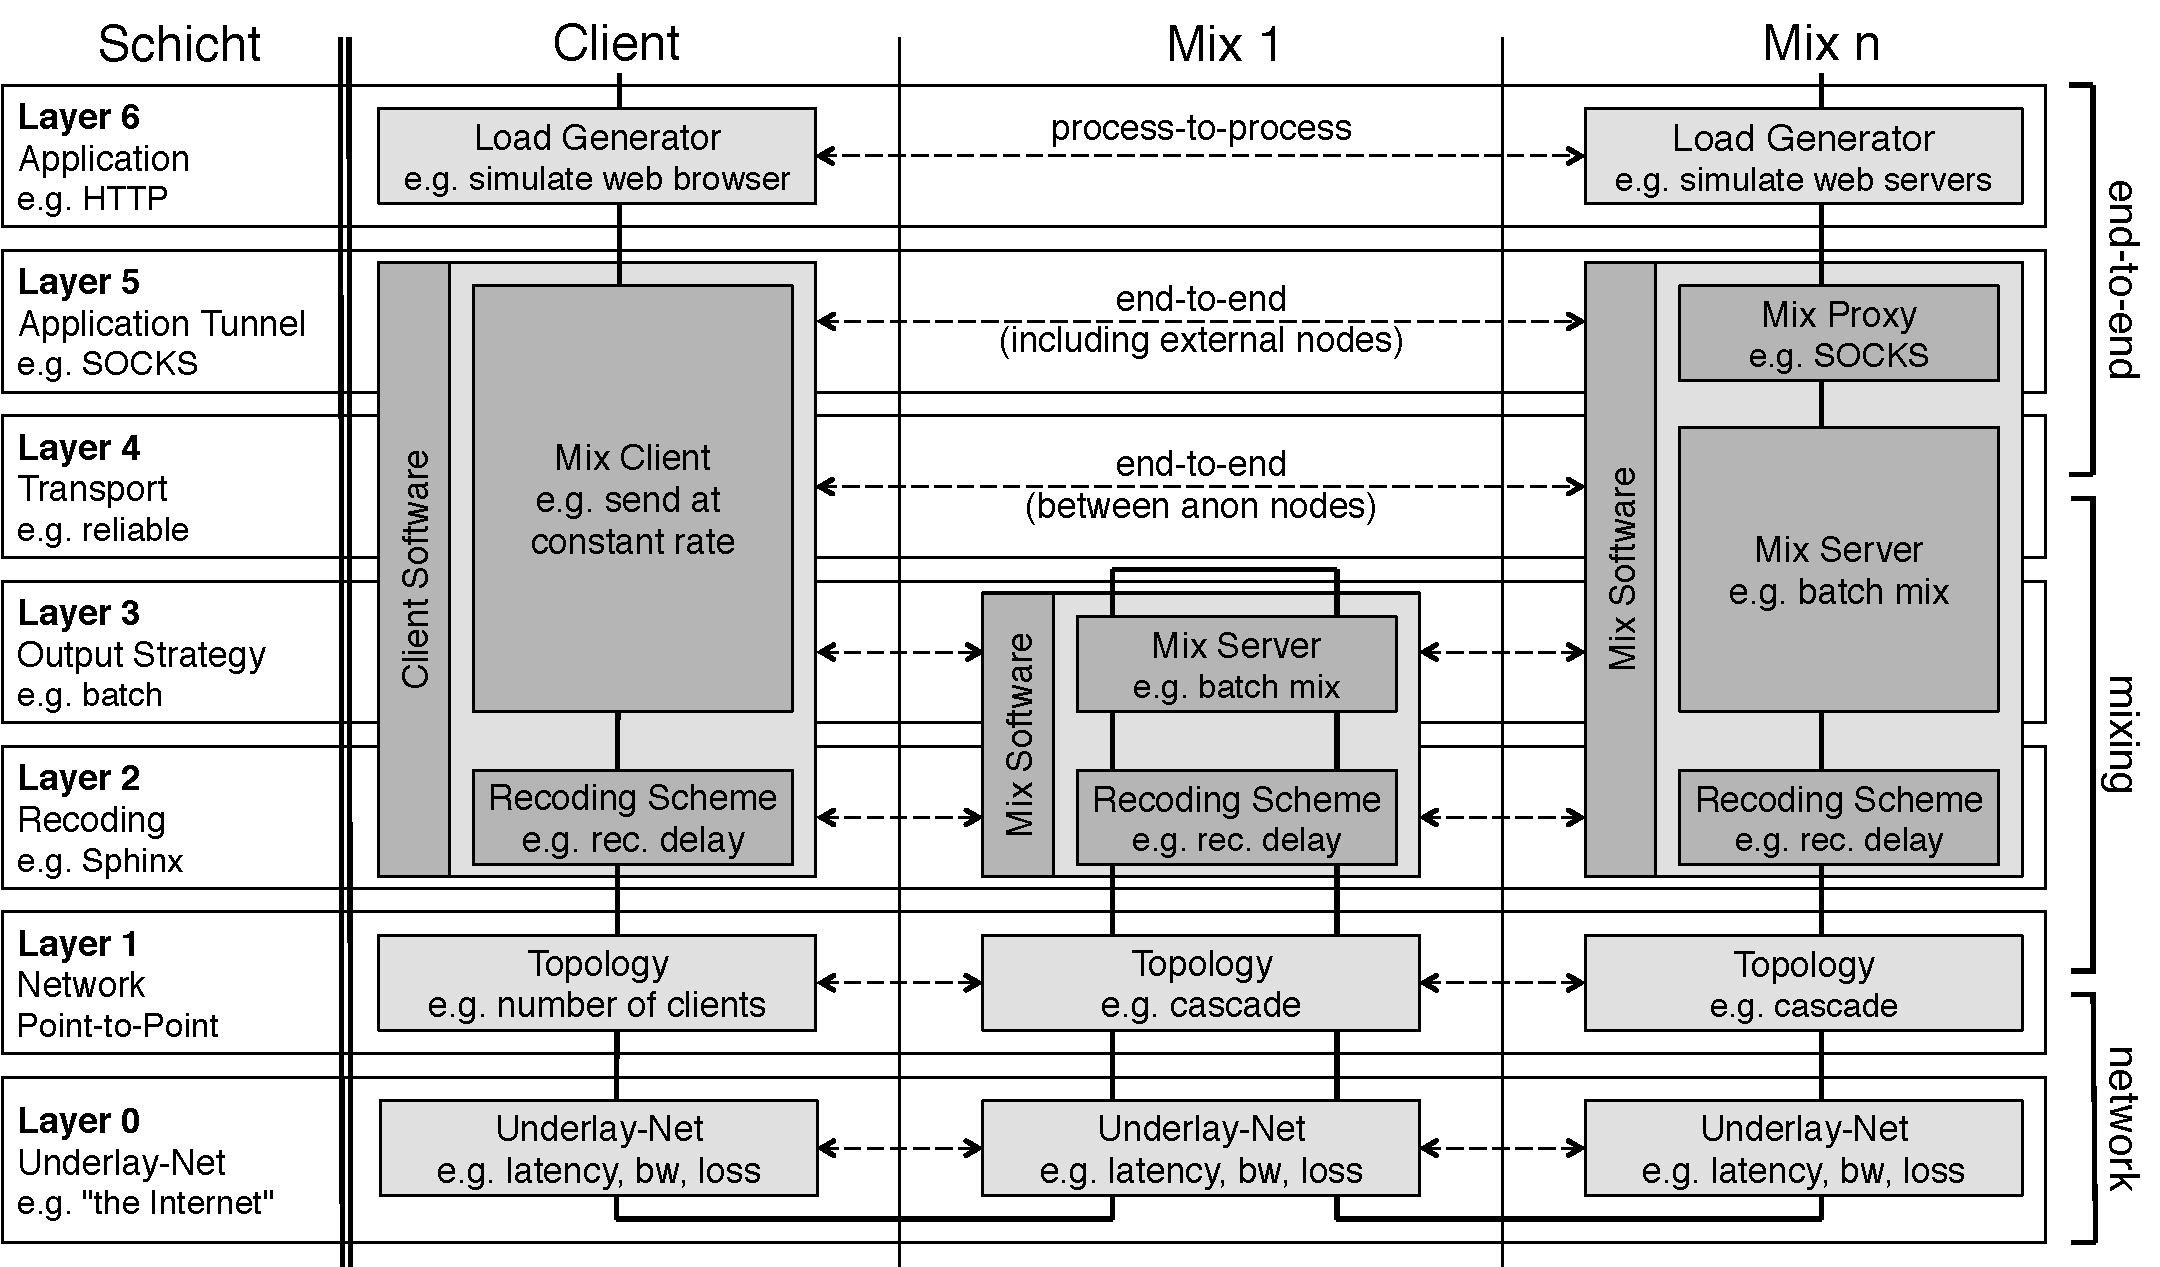
\includegraphics[width=\textwidth]{img/simulatorNamingNew.pdf}
     \caption{gMix-Layer}
     \label{img:gMixLayers}
\end{figure}

Die Kommunikation der einzelnen Layer untereinander erfolgt asynchron und wird vom Framework verwaltet, so dass sich Pluginentwickler nicht um die Details kümmern müssen. Diese Kapselung ist dichter an dem Prinzip eines Protokollstacks und erleichtert das Verständnis und die Modellierung. Jeder Layer wird durch verschiedene Plugins realisiert. Durch die Kapselung sind die Plugins dabei leicht austauschbar um Vergleiche zwischen verschiedenen Strategien und Algorithmen durchführen zu können.
\\

Hauptmerkmal von gMix ist, dass es in der Lage ist, jede dieser Schichten zu simulieren. Der gMix-Simulator kann für jede der Schichten mit verschiedenen Plugins ausgestattet werden, beispielsweise unterschiedliche Ausgabestrategien oder Netzwerktopologien charakterisieren.
Der Simulator wird so verwendet, dass alle notwendigen Informationen in einer Konfigurationsdatei gehalten werden. Eine solche Datei wird für jedes Experiment angelegt und umfasst unter anderem die Auswahl der Plugins, notwendige Parameter oder welche Werte im Laufe des Experimentes variiert werden sollen. Um diese Arbeit zu vereinfachen und zu unterstützen ist die GUI in der Lage diese Experimentdateien zu lesen und zu schreiben, sowie den Simulator mit verschiedenen Experimentdateien zu starten.
% subsection gmix (end)

\subsection{Ziele der GUI} % (fold)ssu
\label{sub:ziele_der_gui}
Die im Rahmen dieser Arbeit erstellte Graphische Benutzeroberfläche (GUI) dient als Erweiterung zum gMix Simulator und soll Benutzer bei verschiedenen Aufgaben unterstützen. Da gMix selbst als ein Werkzeug für Forschung und Lehre entwickelt wurde, sind Benutzer aus diesen Bereichen ebenfalls die Zielgruppe. Die GUI richtet sich in erster Linie an drei Fokusgruppen:
\begin{itemize}
	\item Schüler und Studenten, die an das Konzept von Mixen und ihre Funktionsweise herangeführt werden sollen. Für diese Gruppe soll die GUI vor allem einfach zu bedienen sein und bei der Vermeidung von Fehlern in den Einstellungen helfen.
	\item Forscher, welche gMix verwenden um Simulationen durch zu führen oder neue Implementationen erstellen wollen. Dieser Gruppe soll die Arbeit erleichtert werden, indem die GUI Zur Übersichtlichkeit beiträgt und die Möglichkeit bietet, mehrere Simulationen auf einfache Weise zu verwalten und nacheinander automatisiert ablaufen zu lassen.
	\item Pluginentwickler, die gMix erweitern wollen und eine einheitliche Schnittstelle zum Anbinden ihrer Plugins benötigen. Diese Gruppe profitiert von der Verwendung von Annotationen, welche weiter unten beschrieben wird und der Möglichkeit Abhängigkeiten zwischen Plugins möglichst einfach darzustellen.
\end{itemize}

Die GUI bietet zur Unterstützung im Umgang mit gMix mehrere Funktionen. Zu den offensichtlichsten gehören dabei die erhöhte Übersichtlichkeit, da es nicht mehr notwendig ist, alle Parameter für eine Simulation per in eine Konfigurationsdatei zu schreiben. Dabei werden außerdem nur die Parameter zum einstellen angeboten, die auch möglich und sinnvoll sind, was einige Fehlerquellen bereits im Vorfeld ausschließt. In der GUI  ist außerdem ersichtlich welche Plugins auf welcher Ebene ausgewählt werden können und somit auch welche in Konkurrenz um die selbe Funktion stehen, wodurch Konflikte vermieden werden. Zur einfacheren Verwaltung der Simulationen, ist es möglich diese zu speichern und zu laden, sowie sie in einer Liste vor zu halten, die dann bei der Simulation abgearbeitet werden kann. Zudem können die Ergebnisse der Simulationen in der GUI betrachtet oder als Dateien exportiert werden. Zur Visualisierung wird dabei Gnuplot (www.gnuplot.info) verwendet. Die Beschreibung der GUI geschieht mit Hilfe von Annotationen, welche direkt in den Quelltext des jeweiligen Plugins geschrieben werden. Dadurch brauchen Pluginentwickler nur ihre Java-Klassen erstellen und müssen an keiner anderen Stelle etwas ändern. Eine genauere Behandlung der Annotationen widmet sich Kapitel 3.
% subsection ziele_der_gui (end)

\subsection{Überblick} % (fold)ssu
\label{sub:überblick}
In den folgenden  Kapiteln wird die GUI und ihre Komponenten erläutert, sowohl von der für den Benutzer sichtbaren Seite, als auch von den Designentscheidungen und der Architektur. Diese Dokumentation richtet sich damit an Benutzer von gMix ebenso wie an Entwickler.\\
Das folgende Kapitel 2 geht auf die Benutzung der GUI ein und die einzelnen Komponenten werden beschrieben. Es ist daher für die meisten Benutzer interessant, die mit gMix zum Beispiel im Rahmen von Lehre oder Forschung arbeiten wollen. In Kapitel 3 wird das Konzept der Annotations erläutert, wie sie für das Zusammenspiel von GUI und Plugins genutzt werden und warum sich für die Verwendung dieser Technik entschieden wurde. Dieses Kapitel ist damit vor allem für Pluginentwickler von Interesse. Kapitel 4 befasst sich mit der Architektur der GUI und ihrer Kopplung an den gMix-Simulator. Abschließend hält Kapitel 5 noch weitere Informationen für Entwickler bereit.
% subsection ziele_der_gui (end)


\section{GUI}
\label{sub:guielemente}
Die GUI für den gMix-Simulator wurde wie alle zuvor beschriebenen Elemente mit Java realisiert. Dies garantiert Plattformunabhängigkeit und gleiches Look and Feel auf verschiedenen Systemen. Java bietet drei unterschiedliche Layout Manager an, mit denen sich GUIs realisieren lassen.
\begin{enumerate}
\item JavaFX
\item SWT
\item Swing
\end{enumerate}
Unsere Wahl ist auf Swing gefallen, da dies ein sehr dynamisches Framework zur Erstellung einer GUI ist. JavaFX wurde hauptsächlich für den Einsatz in Webanwendungen entworfen. SWT bietet die Möglichkeiten statische GUIs zu bauen, was man beispielsweise von Produkten wie  Eclipse kennt.\\

Swing ist in der Anordnung von GUI Elementen wie Buttons oder Textfeldern sehr frei und nimmt dem Entwickler große Teile des Layoutings ab. In Swing selbst werden sog. \emph{JPanel} erzeugt, in denen die GUI Elemente angeordnet werden. Die \emph{JPanel} an sich wiederum können Bestandteil eines \emph{JFrame} sein, welches ein einfaches Fenster ist. Die Anordnung der Elemente wird durch das sog. \emph{Layoutmanager} gehandhabt. Beispiele für \emph{Layoutmanager} sind BorderLayout und MigLayout. Das \emph{BorderLayout} ist einer der simpelsten \emph{LayoutManager} von Java Swing. Er unterteilt ein \emph{JPanel} in fünf verschiedene Bereiche

\begin{itemize}
    \item {PAGE\_START}
    \item {PAGE\_END}
    \item {LINE\_START}
    \item {LINE\_END}
    \item {CENTER}
\end{itemize}

Das \emph{MigLayout} ist eine OpenSource Entwicklung, die gerade für große GUI Projekte eine besondere Agilität mit sich bringt. Bei der Verwendung des \emph{MigLayout} werden ähnlich des \emph{GridLayout} Koordinaten für einzelne GUI Elemente angegeben. Verbildlicht bedeutet dies, dass die GUI in ein Raster unterteilt wird. In dieses Raster werden die Elemente angeordnet und mit sog. \emph{Contstraints} versehen. Die \emph{Constraints} garantieren, dass die Elemente den zur Verfügung stehenden Platz nutzen, sich ordentlich orientieren oder sich in einer bestimmten Reihenfolge anordnen. \\

Einige nützliche Standard-Features von Swing wurden ebenso in diesem Projekt verwendet. Dazu gehören Menüs und Shortcuts. Über die Menüs, welche am oberen Rand der Anwendung zu finden sind, lassen sich generelle Einstellungen vornehmen. Dazu zählt beispielsweise das auskoppeln von einzelnen Elementen der GUI (siehe Unterabschnitte \ref{ssub:configview}, \ref{ssub:resultview} und \ref{ssub:helpview}). Die Shortcuts erlauben es dem Nutzer die komplette GUI mit der Tastatur zu bedienen. \\

Abbildungen \ref{fig:gui1} und \ref{fig:gui2} zeigen die fertige GUI des gMix Simulators. Abbildung \ref{fig:gui1} zeigt \emph{Configuration View, Simulation View, Konsole} und \emph{Results View}. In Abbildung \ref{fig:gui2} ist zusätzlich noch der \emph{Help View} zu sehen. Im Weiteren werden die einzelnen Bestandteile der GUI erläutert.

\begin{figure}[!htp]
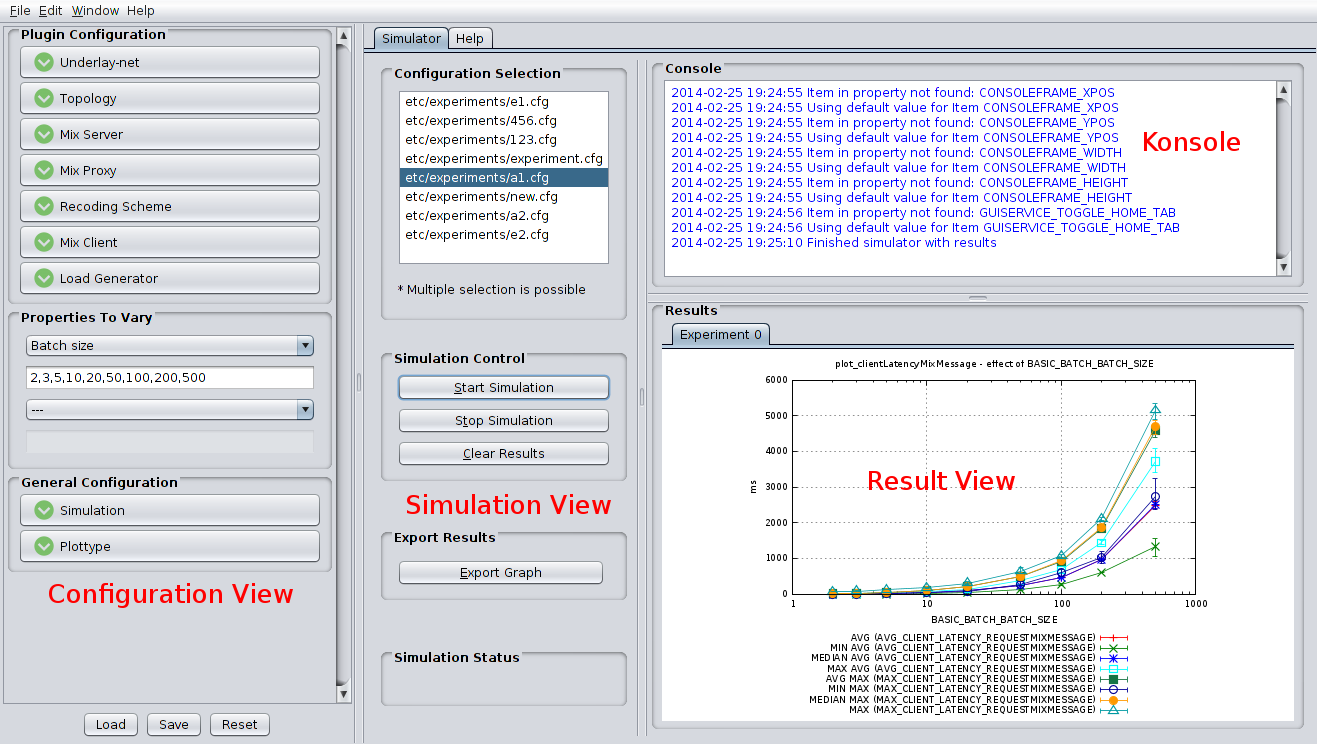
\includegraphics[width=\textwidth]{img/gmixGuiSimulator}
\caption{gMix GUI I}
\label{fig:gui1}
\end{figure}

\begin{figure}[!htp]
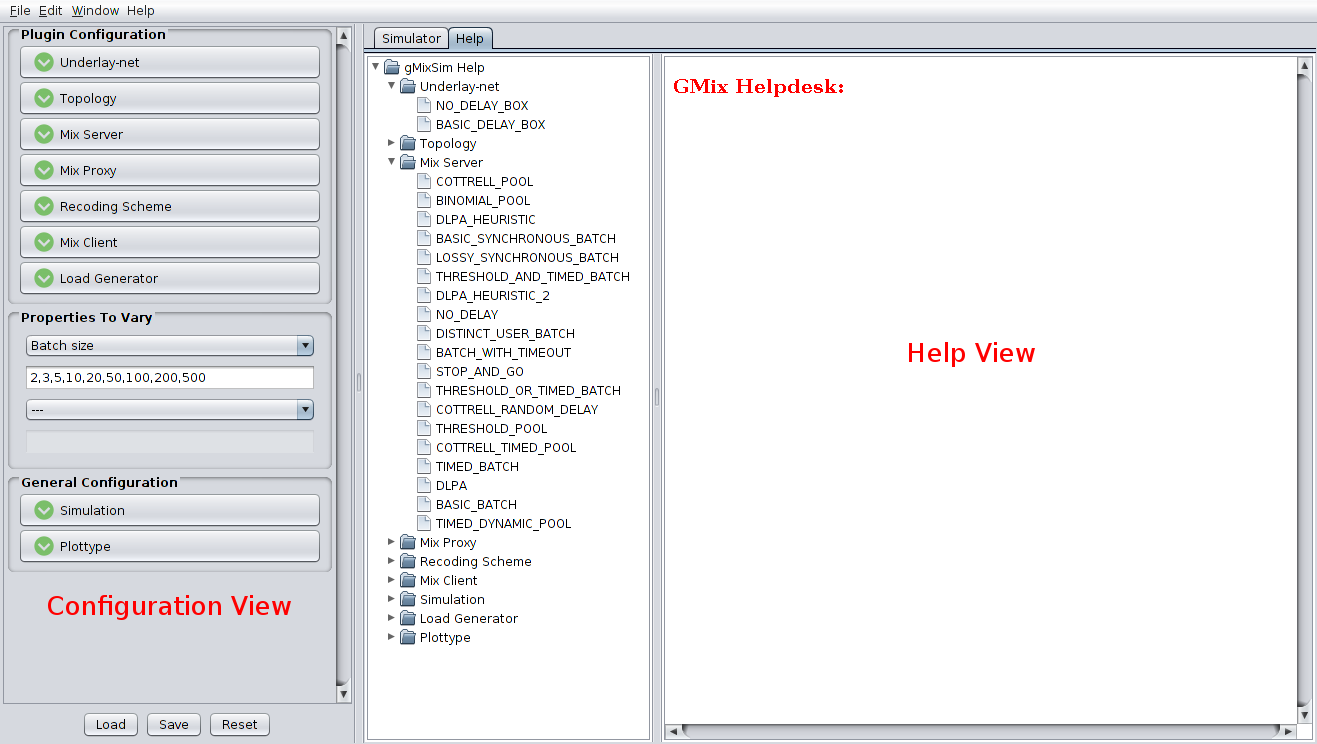
\includegraphics[width=\textwidth]{img/gMixGuiHelp}
\caption{gMix GUI II}
\label{fig:gui2}
\end{figure}

\subsection{Configuration View} % (fold)
\label{ssub:configview}
Der \emph{Configuration View} bildet zusammen mit der \emph{SimPropRegistry} (vgl. \ref{sssub:simpropregistry}) das Herzstück der GUI. Mit ihr hat der Nutzer die Möglichkeit die Simulation auf einfach Art und Weise zu konfigurieren. \\

Der \emph{ConfigurationView} besteht aus den sog. \emph{AccordionEntries}, der \emph{PropertiesToVary} Konfiguration, einer allgemeinen Simulationskonfiguration und den Buttons \emph{Load, Save} und \emph{Reset}. Angelehnt an moderne Smartphone Betriebssysteme wurden die \emph{AccordionEntries} entwickelt, welche sich durch einen Button und darunter verborgene Konfigurationsmöglichkeiten auszeichnen. Jeder Layer der Simulatorkonfiguration lässt sich somit auf einen Button abbilden unter dem ein Plugin für diesen gewählt werden kann. In der vorliegenden Version der gMix-Simulator GUI werden folgende Layer verwendet:
\begin{enumerate}
\item \textbf{Underlay-net}, dass zugrundeliegende Netzwerk
\item \textbf{Topology}, der Aufbau des Netzwerks
\item \textbf{Mix Server}, das Verhalten des Mix Servers
\item \textbf{Mix Proxy}, die Proxykonfiguration
\item \textbf{Recoding Scheme}, die Art der Umkodierung
\item \textbf{Mix Client}, der Client
\item \textbf{Load Generator}, die Verkehrsdatenerzeugung
\end{enumerate}
 Klickt man auf den Button eines \emph{AccordionEntries}, so erhält man zunächst eine Auswahl in Form einer Combobox, um ein Plugin zu wählen. Hat man ein Plugin gewählt, erhält man die Konfigurationsmöglichkeiten für dieses Plugin. Dabei wird die Anzeige dynamisch, ausgehend vom Variablentyp der \emph{SimulationProperty}, erstellt. Der Typ wurde zuvor vom Entwickler per \emph{Annotation} festgelegt. Zwei Beispiele für dynamisch erzeugte Konfigurationsmöglichkeiten sind
 \begin{itemize}
 \item \emph{Integer} wird standardmäßig über einen Spinner konfiguriert. 
 \item \emph{Boolean} wird mit einer Checkbox konfiguriert.
 \end{itemize}
 Diese Konfiguration garantiert es dem Nutzer sofort die Übersicht über seine Konfigurationsmöglichkeiten zu erhalten. Zusätzlich werden Fehlkonfigurationen ausgeschlossen, da die Konfiguration auf deren Variablentypen eingeschränkt ist. Falsche Werteingaben werden mit Hilfe des \emph{DependencyCheckers} (vgl. \ref{sssub:dependencychecker}) verhindert. \\

 Unter der Pluginkonfiguration befindet sich die Konfiguration für die \emph{PropertiesToVary}. Diese geben an, welche Properties bei der Simulation variiert werden sollen. Die Eingabe wird hier über eine simple Textbox realisiert um die Konfiguration möglichst offen zu gestalten. \\

 Den letzten Abschnitt im \emph{Configuration View} bilden die allgemeinen Einstellungen zur Simulation und dem \emph{Plottype}. Diese wurden ebenfalls als \emph{AccordionEntry} dargestellt, um die Übersichtlichkeit zu bewahren. Der Eintrag Simulation bietet beispielsweise die Option den Endzeitpunkt einer Simulation zu konfigurieren. Unter dem \emph{AccordionEntry} \emph{Plottype} lässt sich unter anderem das Plotskript für Gnuplot definieren.\\

 Nach der Konfiguration einer Simulation kann diese über den Button \emph{Save} abgespeichert werden. Dabei werden alle Einstellungen in ein einheitliches Konfigurationsdateiformat gespeichert. Die so generierten Konfigurationsdateien (EDFs) lassen sich einfach wiederverwenden und sind zusätzlich übersichtlich gestaltet. Über den Button \emph{Load} lässt sich eine so zuvor gespeicherte EDF wieder öffnen und in den \emph{Configuration View} laden. Dabei werden alle \emph{AccordionEntries} aufgeklappt um eine direkte Übersicht über die Konfiguration zu zeigen. Der Button \emph{Reset} setzt die Einstellungen auf eine Standardkonfiguration zurück. Möchte man eine definierte Konfiguration ausführen, so muss diese zuvor als EDF gespeichert werden, um im Simulation View (in Abschnitt \ref{ssub:simulationview} erläutert) auswählbar zu sein.\\

 Zur Unterstützung der Übersichtlichkeit bietet die GUI die Möglichkeit den \emph{Configuration View} vom Hauptfenster auszukoppeln. Dies ist besonders hilfreich wenn man z.B. mit mehreren Monitoren arbeitet oder das Hauptfenster ohne die Konfiguration betrachten möchte. Dabei wird ein neues Fenster erzeugt, welches nur den \emph{Configuration View} enthält.

\subsection{Simulation View} % (fold)
\label{ssub:simulationview}
Der \emph{Simulation View} lässt den Nutzer seine vorher gespeicherte Konfiguration ausführen und generiert direkt einen Graphen mittels Gnuplot. Dadurch sind die Ergebnisse der Simulation sofort einzusehen. Der \emph{Simulation View} besteht aus drei Komponenten. Auf der linken Seite sind die vorhandenen Konfigurationsdateien zu sehen. Diese können per Multiselect (d.h. mehrere auf einmal) in der \emph{Configuration Selection} ausgewählt werden. Mit Hilfe der \emph{Simulation Control} kann die Simulation gestartet (\emph{Start Simulation}) oder angehalten (\emph{Stop Simulation}) werden. Die generierten Ergebnisse können mittels \emph{Clear Results} gelöscht werden. Zur Laufzeit des Programms werden die generierten Dateien jedoch nicht gelöscht, sondern nur aus der Anzeige entfernt. Über \emph{Export Results} lassen sich generierte Graphen in zwei verschiedenen Formate exportieren. Zur Verfügung stehen .png und .eps. Beim Start einer Simulation erscheint im \emph{Simulation Status} ein Fortschrittsbalken, der signalisiert, dass die Simulation im Gange ist. \\

Auf der rechten Seite des \emph{Simulation View} befindet sich in der oberen Hälfte die Konsole (siehe \ref{ssub:consoleview}). Darunter ist der \emph{Result View} (siehe \ref{ssub:resultview}) angesiedelt.

\subsection{Result View} % (fold)
\label{ssub:resultview}
Der \emph{Result View} präsentiert die Ergebnisse der zuvor ausgewählten Simulation. In der vorliegenden Version der gMix Simulator GUI wird Gnuplot zum Rendern der Ergebnisse verwendet. Nach erfolgreicher Simulation wird im \emph{Result View} ein Tab erzeugt, der den dazugehörigen Graphen anzeigt. Ergebnisse werden in der Reihenfolge generiert, wie sie von oben nach unten in der Liste der \emph{Configuration Selection} ausgewählt wurden. Zusätzlich gibt die Legende der Graphen Auskunft, um welche Simulation es sich handelt. Die Ergebnisse werden mittels des zuvor definierten Plotskripts erstellt. Gnuplot liefert das Ergebnis als Vektorgrafik, damit diese in der GUI ordentlich skalieren. Über die in \ref{ssub:simulationview} beschriebene Funktion lässt sich der Graph auch in andere Formate exportieren und speichern. Löschen lassen sich erstellte Ergebnisse mit Hilfe des Buttons \emph{Clear Results}. Um die Ergebnisse vergrößert zu betrachten genügt ein Rechtsklick auf das Ergebnis um über das Menü den Graphen von der GUI zu entkoppeln. So können mehrere Ergebnisse gleichzeitig vergrößert, entkoppelt und gegeneinander gestellt werden. 

\subsection{Konsole} % (fold)
\label{ssub:consoleview}
Die \emph{Konsole} der gMix Simulator GUI gibt Auskunft über den aktuellen Status der GUI und den Fortschritt der Simulation. Speziell für diese Zwecke wurde der Logger \emph{log4j} von Apache um einen Appender erweitert, welcher bei einem bestimmten Loglevel in die \emph{Konsole} schreibt. Somit lassen sich die Nachrichten auf der \emph{Konsole} von Nachrichten, die in logs gespeichert werden unterscheiden.

\subsection{Help View} % (fold)
\label{ssub:helpview}
Der \emph{Help View} bietet dem Anwender Unterstützung bei der Benutzung der GUI. Ausgehend von den registrierten Plugins wird die Hilfe, angelehnt an die Anordnung der \emph{AccordionEntries}, aufgebaut. Dabei entsteht eine Baumstruktur, die mittels \emph{JTree} umgesetzt wurde. Als Blätter des \emph{JTree} werden die verfügbaren Plugins aufgezeigt. Wählt man ein Element aus öffnet die GUI eine HTML-Datei, welche zuvor vom Pluginentwickler angelegt wurde. Dabei ist zu beachten, dass die HTML-Datei den gleichen Namen wie der Plugin-Key hat. Somit werden Kollisionen vermieden und eine eindeutige Zuordnung von Plugin zu Hilfe erstellt. Der \emph{Help View} lässt sich wie der \emph{Configuration View} auskoppeln, um das gleichzeitige Arbeiten an der Simulation und Nachschlagen in der Hilfe zu erleichtern.

\subsection{Bedienungsablauf in der GUI}
\label{ssub:bedienung}
In der Reihenfolge der zuvor aufgezählten GUI Elemente lässt sich einfach eine Simulation durchführen. Für den schnellen Einstieg folgt ein HowTo:

\begin{enumerate}
\item \textbf{Auswahl der Plugins:} \newline Der Benutzer wählt im \emph{Configuration View} die gewünschten Plugins mit Hilfe der \emph{AccordionEntries} aus und konfiguriert diese.
\item \textbf{Auswahl der Properties To Vary:} \newline Anschließend werden die zu variierenden Werte angegeben.
\item \textbf{Simulationskonfiguration:} \newline In der \emph{General Configuration} werden Angaben zum Ende der Simulation und Plotskript gemacht.
\item \textbf{Speichern der Konfiguration:} \newline Über den Button \emph{Save} wird die vorgenommene Konfiguration gespeichert.
\item \textbf{Auswahl der zu simulierenden Konfiguration:} \newline Die soeben gespeicherte Konfiguration wird in der \emph{Configuration Selection} ausgewählt. Dank Multiselection können auch mehrere Konfigurationen gleichzeitig gewählt werden.
\item \textbf{Start der Simulation:} \newline Durch Druck auf den Button \emph{Start Simulation} wird die Simulation gestartet und anschließend werden die Ergebnisse im \emph{Results View} ausgegeben. 
\end{enumerate}

\section{Designentscheidungen} % (fold)
\label{sec:designentscheidungen}

\subsection{XML vs. Annotations} % (fold)
\label{sub:xml}
In diesem Abschnitt werden wir kurz motivieren, warum wir uns bei der Entwicklung der gMix GUI für die Verwendung Annotationen und nicht für die Verwendung XML entschieden haben. Vorher werden wir jedoch kurz erörtern warum wir in dem GUI Projekt eine Beschreibungssprache wie Annotations (oder XML benötigen) benötigt werden.\\

Da der gMix Simulator pluginbasiert ist, wäre es für den Entwickler unpraktisch eine GUI statisch zu programmieren. Stattdessen ist es in einem solchen Projekt wünschenswert, dass sich die GUI generisch aufbaut. Hierzu bietet es sich an eine Technik zu verwenden, die es erlaubt pluginabhängige Metadaten (wie Informationen über GUI-Elemente) zu beschreiben. Diese Daten können dann beim Starten der GUI (abhängig von den vorhandenen Plugins) an vordefinierten Stellen ausgelesen werden. Ein spezieller Programmabschnitt, der für die Generierung der GUI-Elemente zuständig ist, verarbeitet anschließend die Informationen und erstellt eine einheitliche GUI.\\

Zwei häufig verwendete Techniken zur Beschreibung von Metadaten sind Annotationen und XML. Bei der GUI für den gMix Simulator haben wir uns bewusst für die Verwendung von Annotationen entscheiden. Es folgt nun die Begrüngung:\\

Flexibilität / Erweiterbarkeit: Ein sehr wichtiger Aspekt ist, dass das von uns angestrebte Annotationen-System sehr einfach erweiterbar sein soll. Da der \emph{gMix-Simulator} Plugin-basiert ist, kann es zu einem späteren Zeitpunkt (nach Projektende) notwendig sein, dass \emph{Properties} oder \emph{Plugins} beispielsweise um neue Eigenschaften erweitert werden sollen. Während im Falle von XML ggf. das Schema angepasst werden muss und/oder komplexere Eingriffe in das Parsing notwendig sein können, ist der Aufwand bei der Verwendung von Annotationen sehr gering. Hier genügt es die jeweiligen Annotationen (beispielsweise \emph{IntSimulationProperty}), um die gewünschten Felder zu erweitern. Die zugehörigen POJOs (beispielsweise \emph{IntProp}), welche später die Informationen aus den Annotationen enthalten, müssen dann lediglich um \emph{Getter} und \emph{Setter} erweitert werden. Die notwendigen Änderungen am Annotations-Parser (in der Klasse \emph{SimPropRegistry}) sind ebenfalls sehr einfach und beschränken sich auf das Auslesen der Annotation und das Aufrufen der \emph{Setter} der jeweiligen POJOs.\\

Dezentralisierung: Im Gegensatz zu XML werden Annotationen direkt in den Plugin-Code eingebettet. Dieses bringt gleich zwei Vorteile mit sich. Zum einen werden dadurch zentrale Dateien vermieden, wodurch eine sehr lose Kopplung ermöglicht wird, wie sie bei Plugin-Systemen wünschenswert ist --- Versionskonflikte von zentralen Dateien werden so vermieden. Dieses ist bei Plugin-System sehr wichtig. Allerdings wäre eine lose Kopplung auch noch mit XML möglich, würde jedoch unweigerlich in einer großen Anzahl an XML-Dateien enden, sofern jedes Plugin eine eigene XML Datei erhält. Der zweite Vorteil ist, dass ein Pluginentwickler die Festlegung der Eigenschaften von Properties und Plugins genau dort vornimmt, wo diese auch logisch gesehen hingehören. Nämlich direkt an den Properties und den Plugins selbst. Dieses ist gerade bei der Entwicklung neuer Plugins von Vorteil, da nicht permanent zwischen mehreren Dateien (Java Code und XML Datei) hin und her gesprungen werden muss. Bei der Erweiterung von existierendem Code kann dieses jedoch auch nachteilig sein, da ein unerfahrener Entwickler ggf. erst nach der relevanten Stelle im Code suchen muss und nicht wie bei XML alle Informationen in einer bekannten Datei vorliegen hat.

Ein dritter Aspekt ist, dass Annotationen ein Teil der Sprache Java sind. Dieses bedeutet für einen Entwickler, dass er bei den Programmieraufgaben mehr Unterstützung durch die IDE bekommt, als es bei XML möglich ist. So wird er bei der Erweiterung von Annotationen beispielsweise frühzeitig auf syntaktische und semantische Fehler aufmerksam gemacht. Bei der Verwendung von XML ist dieses nicht gegeben, da zwischen der XML-Datei und Java-Code kein syntaktischer Zusammenhang besteht. Die Erkennung von semantischen Fehlern ist bei XML dadurch eingeschränkt, da XML-Code keine Typen kennt und somit nicht erkennen kann, ob eine Eingabe valide ist oder nicht. Auch die automatische Komplettierung funktioniert zusammen mit den Annotationen.\\

Für den Anwender der GUI ist die Wahl zwischen Annotationen und XML irrelevant, da dieses aus Benutzersicht transparent ist. Der Pluginentwickler profitiert jedoch im Normalfall ein klein wenig mehr von dem Einsatz von Annotationen. Aus diesem Grund haben wir uns entschieden ein neues Framework (basierend auf Annotationen) zu entwickeln und nicht auf ein (aus einem früheren Projekt verfügbaren) XML basierendes Framework zurückzugreifen.

% subsection xml (end)

% section einleitung (end)

\newpage
\subsection{Annotations (Entwickler Informationen)} % (fold)
\label{sub:annotations}
Dieser Abschnitt beschreibt die unterschiedlichen Typen von Annotation, welche unsere GUI verwendet. Insgesamt gibt es drei unterschiedliche Typen von Annoationen, die in der GUI zum Einsatz kommen. Es werden nun die einzelnen Typen motiviert und ihre Unterschiede erläutert. Weiterhin wird ausführlich auf die einzelnen Felder der Annotationen eingegangen.\\

Zuvor soll der Leser jedoch mit den von uns verwendeten Bezeichnungen, in Bezug auf die GUI-Elemente, bekannt gemachet werden. Hierzu dient die nachfolgende Abbildung \ref{fig:guielements}. 

\begin{figure}[!htp]

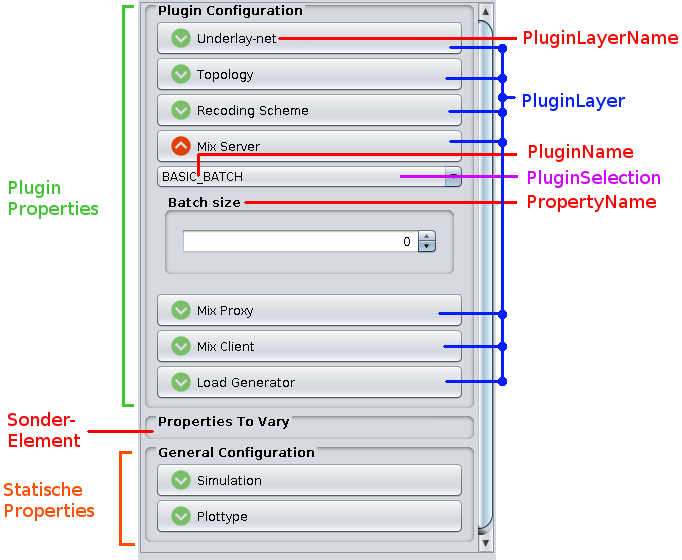
\includegraphics[scale=0.56]{img/configtool_edit.png}
% subsection annotations (end)

\caption{Ausschnitt des 'Config Tools'}
\label{fig:guielements}
\end{figure}

Bevor es die gMix GUI gab, wurde die Konfiguration des Simulators in einer Textdatei (EDF - Experiment Definition File) vorgenommen. Ein Auszug aus einer solchen Konfigurationsdatei ist in Listing \ref{lst:edf} dargestellt. 

\newpage

\begin{lstlisting}[caption={Auszug aus einer Simulator Konfiguration},label=lst:edf,frame=lrtb]
#-OUTPUT_STRATEGY--OR--FLUSHING_ALGORITHM----------
# ...
# Some possible values: NO_DELAY, ... 
# BATCH_WITH_TIMEOUT, BINOMIAL_POOL, ... 
# COTTRELL_TIMED_POOL, DISTINCT_USER_BATCH, ... 
# DLPA_HEURISTIC_2, LOSSY_SYNCHRONOUS_BATCH, ...
# THRESHOLD_AND_TIMED_BATCH, THRESHOLD_OR_TIMED_BATCH 
# TIMED_BATCH, TIMED_DYNAMIC_POOL
#	
OUTPUT_STRATEGY = BASIC_BATCH
...
BASIC_BATCH_BATCH_SIZE = 100
...
\end{lstlisting}

Eine Hauptaufgabe unserer Arbeit bestand nun darin eine geeignete Abbildung zu finden, die es erlaubt, die Inhalte einer solchen Konfigurationsdatei grafisch darzustellen. Es zeigte sich, dass hierfür eine hierarchische Struktur mit drei Ebenen geeignet ist (vergleiche Abb. \ref{fig:guielements}).

\begin{itemize}
	\item (Plugin)Layer: Die Auswahl des Layers legt fest, welches Plugin als Implementation für einen bestimmten Software-Layer während der Simulation verwendet werden soll. Die einzelnen Layer des gMix Simulators können in Abschnitt \ref{sub:gmix} nachgelesen werden. 
	\item Plugin: Unter eine, Plugin wird eine in sich geschlossene Implementation einer bestimmten Funktionalität verstanden. Jeder Layer setzt eine gewisse Schnittstelle (für die auf dem Layer agierenden Plugin) voraus, legt dabei jedoch nicht fest, wie die Implementation selbst auszusehen hat.
	\item Property: Je nach Implementation benötigt ein Plugin Parameter, um gewisse interne Variablen zu konfigurieren. Anzahl, Typ und zulässige Werte dieser Parameter hängen jedoch mit der Implementation des Plugins zusammen und müssen von dem Experimentator festgelegt werden. Zu diesem Zweck muss ein Plugin je Parameter eine Property definieren, die der Experimentator schließlich in der GUI setzen darf.
\end{itemize} 

Die Terminologie welche wir für die EDF verwenden ist die gleiche wie zuvor, nur dass es dort keine \emph{Namen (names)} sondern \emph{Schlüssel (keys)} gibt. Der Unterschied ist, dass sich Namen immer auf die Darstellung innerhalb von GUI-Elementen beziehen, währen sich \emph{Schlüssel} auf die eindeutigen Strings in den EDFs beziehen.

Im Listing \ref{lst:edf} ist 'OUTPUT\_STRATEGY' der PluginLayerKey (kurz: LayerKey) für das Plugin, welches auf der Ebene \emph{Output Strategy} (EDF) bzw.  \emph{Mix-Servers} (GUI) argiert. In der EDF bildet der LayerKey auf ein PluginKey ab (hier 'BASIC\_BATCH') und identifiziert damit das aktive Plugin. Das Plugin, welches den PluginKey 'BASIC\_BATCH' zugewiesen ist, hat wiederum eine Property, welche durch den PropertyKey 'BASIC\_BATCH\_BATCH\_SIZE' identifiziert wird (Dieses geht jedoch nicht aus der EDF hervor, sondern ist im Code des Simulators bzw. der Plugins definiert).\\

Nachdem nun die grundlegenden Terminologien eingeführt wurden, wollen wir die Annotationen genauer betrachten, welche den Aufbau der GUI bestimmen. Wir gehen dabei \emph{bottom-up} vor, da weniger Informationen vorweggenommen werden müssen und die Argumentation somit für den Leser ein wenig verständlicher sein sollte.

\subsubsection{Property Annotation} % (fold)
\label{ssub:feld_annotation}
Die Property Anotationen sind wohl die wichtigsten und auch komplexesten Annotationen, die wir in der GUI verwenden. Diese Art von Annotationen werden dazu verwendet, um Felder im Quellcode des Simulators und im Quellcode der Plugins zu annotieren. Dabei werden solche Felder annotiert, die tatsächlich Simulation-Properties halten. Diese sind daran zu erkennen, dass ihr Wert über \emph{Simulator.settings.getProperty()} abgefragt wird, um den Simulator oder ein Plugin zu parametrisieren.\\

Alle \emph{Properties} haben eine gewisse Grundmenge an Feldern, die in der folgenden Auflistung erläutert werden. Besonders sei hier die Ausprägung \emph{BoolSimulationProperty} hervorgehoben. Dieses ist die einzige Property Annotation, die außer der folgenden Grundmenge keine weiteren Felder besitzt.
\begin{itemize}
	\item \emph{name:} Es handelt sich um einen String, der den Namen der Property festlegt, wie er in der GUI angezeigt werden soll. Analog zur obigen Grafik entspricht dieses dem \emph{PropertyName}.\\
	\emph{Default:} keinen (Der Entwickler muss diesen Wert händisch setzen)
	\item \emph{key:} Ein String der die Property innerhalb der Experiment-Konfiguration eindeutig identifiziert. Analog zum obigen Listing entspricht dieses dem \emph{PropertyKey}).\\
	\emph{Default:} keinen (Der Entwickler muss diesen Wert händisch setzen)
	\item \emph{position:} Dieses ist ein Integer (>= 0), der die Position des zugehörigen GUI-Elementes steuert. Je kleiner der Wert desto weiter unten taucht das GUI-Element der jeweiligen Proerty auf. Sollten zwei Properties eines Plugins hier den selben Wert haben, so wird lexikalisch geordnet.\\
	\emph{Defalut: 0}\\
	\item \emph{tooltip:} Dieses ist ein String, der angezeigt wird, wenn sich die Maus über dem entsprechenden GUI-Element befindet.\\
	\emph{Default:} leerer String 
	\item \emph{info:} Ein String der (sofern festgelegt) als Infotext an dem entsprechenden GUI-Element der Property auftaucht.  
	\emph{Default: leerer String}
	\item \emph{global:} Ein Boolean über das festgelegt werden kann, ob die Property global (im gesamten PluginLayer) angezeigt werden soll.\\
	\emph{Default:} false
	\item \emph{inject:} Ein String der es erlaubt Properties an eine beliebige Stelle in der GUI zu injizieren. Dieses ist notwendig, wenn Properties beispielsweise zu einem pseudo Plugin gehören (\emph{'Recoding Scheme'} ist z.B. ein solches pseudo Plugin, das in Wirklichkeit nicht als Plugin existiert sondern viel Mehr direkt im Simulator integriert ist. Dem Benutzer soll es jedoch als Plugin dargestellt werden). \\
	\emph{Syntax:} \"{}<LayerPosition>:<LayerKey>,<LayerName> [@<PluginPosition>:<PluginKey>,<PluginName>]\"{}\\
	Wird hier der optionale Plugin-Teil weggelassen, so gilt die Property layerweit als sichbar (global).\\
	\emph{Default:} leerer String (keine Injection)
	\item \emph{isStatic:} Ein Boolean das angibt, ob eine Property im Abschnitt "Plugin Properties" (\emph{Plugin Configuration}) auftauchen soll oder aber im Abschnitt für statische Properties (\emph{General Configuration}). Dieses Feld wird nur in Kombination mit dem Feld \emph{inject} verwendet. Sinnvoll ist der Einsatz meist dort, wo es sich um Properties handelt, die nicht zu einem Plugin gehören und aus logischer Sicht auch nicht auf einer Pluginschicht liegen.\\
	\emph{Default:} false (Property wird in der \emph{Plugin Configuration} angezeigt)
	\item \emph{value\_requirements:} Eine Klasse, welche von der abstrakten Klasse Requirement erbt und in der für diese Property relevante Werte-Anforderungen umgesetzt werden.
	\item \emph{enable\_requirements:} Eine Klasse, welche von der abstrakten Klasse Requirement erbt und in derer für diese Property relevante Freischalte-Anforderungen umgesetzt werden.
\end{itemize}

Die Annotationen für die numerischen \emph{Properties} (\emph{IntSimulationProperty}, \emph{FloatSimulationProperty} und \emph{DoubleSimulationProperty}) haben neben den Standardfeldern noch weitere Felder, welche hauptsächlich den gültigen Wertebereiche betreffen.
\begin{itemize}
	\item \emph{min:} Ein numerischer Wert (abhängig vom konkreten Typ der Annotation), der den Minimalwert angibt, den die Property annehmen kann. Der angegebene Wert wird von der GUI dazu verwendet, um Benutzereingaben auf ihre Gültigkeit zu prüfen.\\
	\emph{Default:} Integer.MIN\_VALUE bzw. Float|Double.NEGATIVE\_INFINITY
	\item \emph{max:} Ein numerischer Wert (abhängig vom konkreten Typ der Annotation), der den Maximalwert angibt, den die Property annehmen kann. Der angegebene Wert wird von der GUI dazu verwendet, um Benutzereingaben auf ihre Gültigkeit zu prüfen.\\
	\emph{Default:} Integer|Float|Double.MAX\_VALUE
	\item \emph{guiElement:} Ein String durch den festgelegt werden kann, über was für ein GUI-Element der Wert der Property in der GUI konfiguriert werden kann. Aktuell sind für Ganzzahl und Gleitkomma zahlen die beiden Elemente JSpinner (\emph{\"{}spinner\"{}} für Integer, Float und Double) und JSlider (\emph{\"{}slider\"{}} für Integer) implementiert. Beide Elemente verwenden die durch die Felder \emph{min} und \emph{max} festgelegten Grenzen und schützen den Benutzer vor Fehleingaben.\\
	\emph{Default:} \emph{\"{}spinner\"{}} (JSpinner)
	\item \emph{stepSize:} Ein numerischer Wert (abhängig vom konkreten Typ der Annotation), der die Schrittweite eines JSpinners angibt. Dieses Feld ist in Kombination mit \emph{guiElement=\"{}spinner\"{}} sinnvoll, um die Schrittweite manuell festzulegen. So ist es bei einigen Properties vlt. besser eine Schrittweite von 0.1 zu haben, während bei anderen Properties vielleicht kleinere Schrittweiten wie 0.001 besser passen.\\
	\emph{Default:} Integer 1, Gleitkomma 0.001f
	\item \emph{enableAuto:} Ein Boolean durch das festgelegt werden kann, dass die eigentlich numerische Property den String \"{}AUTO\"{} annehmen kann. Der Simulator sieht dieses für einige Properties vor. Im Falle, dass eine numerische Property den Wert \"{}AUTO\"{} hat, wird der tatsächliche Wert automatisch anhand von anderen Properties bestimmt. Wird dieses Feld auf true gesetzt, so gibt es im entsprechenden GUI-Element eine Checkbox, über die der Benutzer festlegen kann, dass die Property automatisch bestimmt werden soll. Für denn Fall, dass  die Checkbox aktiviert ist, wird das eigentliche Eingabeelement (siehe \emph{guiElement}) ausgegraut.\\
	\emph{Beispiele:} Request und Reply Size in ParetoClient, PoissonClient, RequestReplyClient und SendConstantClient\\
	\emph{Default:} false (keine Checkbox für \"{}AUTO\"{}) 
	\item \emph{enableUnlimited:} Ein Boolean durch das festgelegt werden kann, dass die eigentlich numerische Property den String \"{}UNLIMMITED\"{} annehmen kann. Dieses funktioniert analog zu \emph{enableAuto}.\\
	\emph{Beispiel:} DelayBox alle sechs Bandwidth-Properties\\
	\emph{Default:} false (keine Checkbox für \"{}UNLIMITED\"{})
\end{itemize}

Die Annotation \emph{StringSimulationProperty} hat ebenfalls zusätzliche Felder.
\begin{itemize}
	\item \emph{possibleValues:} Ein String über den vordefinierte Werte festgelegt werden können. Die einzelnen Werte werden innerhalb des Strings durch Kommata separiert. Ist dieser String ungleich dem leeren String, so wird die GUI dem Benutzer eine JCombobox zur Manipulation des Wertes der Property anbieten (es sei denn, dass \emph{multiSelection=true} ist, siehe nächstes Feld).\\
	\emph{Default:} leerer String
	\item \emph{multiSelection:} Ein Boolean durch den festgelegt werden kann, dass eine Mehrfachauswahl der vordefinierten Werte möglich ist. Ist dieses Feld auf true gesetzt und sind mittels \emph{possibleValues} mehrere vordefinierte Werte angegeben, so wird ein, auf einer JList basierendes GUI-Element erstellt, das eine Mehrfachauswahl erlaubt.\\
	\emph{Default:} false (Mehrfachauswahl ist deaktiviert) 
	\item \emph{regex:} Ein String der als ein regulärer Ausdruck interpretiert wird. Dieser Ausdruck wird dazu verwendet, um Benutzereingaben auf Gültigkeit zu prüfen (kann ggf. auch sinnvoll in den \emph{ValueRequirements} verwendet werden)\\
	\emph{Default:} leerer String
\end{itemize}

% subsubsection feld_annotation (end)

\subsubsection{Plugin Annotation} % (fold)
\label{ssub:plugin_annotation}
Neben den \emph{Property Annotationen} gibt es zwei weitere Typen von Annotationen. Hierzu gehören unter anderem die \emph{Plugin Annotationen}. Die Einführung dieser Annotationen erschien uns aus dem Grund sinnvoll, da es für einen Pluginentwickler vorteilhaft ist, wenn dieser Eigenschaften, die logisch gesehen zu einem Plugin gehören, auch direkt am Plugin setzten kann. Beispiele hierfür sind der Pluginname, der in der GUI auftaucht (z.B. ''Basic delay box'') oder aber der Schlüssel, unter dem das Plugin in der Experiment-Konfiguration auftaucht (z.B. ''BASIC\_DELAY\_BOX''). Des weiteren erlaubt eine Annotation auf Pluginebene das pluginweite setzen von Eigenschaften. So kann beispielsweise über eine \emph{Property Annotation} festgelegt werden, dass alle Properties, welche in einem Plugin liegen global sind, wodurch sich der Pluginentwickler ggf. ein wenig Schreibarbeit sparen kann. \emph{Property Annotations} haben folgende Felder:

\begin{itemize}
	\item \emph{pluginName:} Ein String, der den Namen festlegt, unter dem das Plugin in der GUI auftritt. Entspricht der bereitgestellt String dem leeren String, so wird stattdessen \emph{pluginKey} als angezeigter Name in der GUI verwendet.\\
	\emph{Default:} Der leere String
	\item \emph{pluginKey:} Ein String, der dem Namen festlegt, unter dem das Plugin in der EDF auftritt. Dieser String muss dabei genau dem String entsprechen, der das Plugin gegenüber dem den \emph{gMix-Simulator} identifiziert (siehe Enums in \emph{evaluation.simulator.pluginRegistry}).
	\item \emph{pluginLayerKey:} Ein String, der den Layer (also die Kategorie) festlegt, unter dessen Pluginauswahl das Plugin auftauchen soll. Dieses Feld ist dafür gedacht, dass der Entwickler von Hand festlegen kann, in welchem Layer das Plugin aufgelistet wird. Dieses ist notwendig, wenn ein Plugin aus mehreren Klassen besteht die keine gemeinsame Oberklasse besitzen. Ein Beispiel für die Anwendung dieses Feldes ist in der Klasse \emph{StopAndGoMessage} zu finden. Dort wird mittels dieses Feld mitgeteilt, dass dieses Plugin in den Layer \"{}OUTPUT\_STRATEGY" gehört. Der Layer selbst wird aber durch die \emph{Plugin Superclass Annotation} in \emph{OutputStrategyImpl} erstellt, welches eine Oberklasse von \emph{StopAndGo} ist. \\
	\emph{ACHTUNG:} Hier dürfen tatsächlich nur Keys eingetragen werden, die auch in einer \emph{Plugin Superclass Annotation} festgelegt wurden. Anderenfalls kommt es zu Fehlern!\\
	\emph{Default:} leerer Sting (automatische Erkennung via \emph{Plugin Superclass})
	\item \emph{documentationURL:}
	Ein String der den Pfad/Dateiname zu der Dokumentation des Plugins. Sofern hier ein Wert angegeben wird (und die referenzierte Datei existiert), wird die Dokumentation in das Menü des \emph{Help Views} aufgenommen.\\
	\emph{Default:} leerer Sting (keine Dokumentation verfügbar)
	\item \emph{visible:} Ein boolean durch das festgelegt werden kann, ob das Plugin in der Pluginauswahl sichtbar ist oder nicht\\
	\emph{Default:} true (sichtbar)
	\item \emph{global:} Ein boolean durch das alle Properties, die zu dem Plugin gehören, gobal gesetzt werden können. Global bedeutet eine Property taucht für jede Pluginwahl in der GUI auf.\\
	\emph{Default: false} (nicht global)
	\item \emph{allowGlobalFields:} Ein boolean durch das festgelegt wird, ob Properties aus dem Plugins global sein dürfen. Global bedeutet eine Property taucht für jede Pluginwahl in der GUI auf.\\
	\emph{Default:} true (globale Properties sind erlaubt)
\end{itemize}
% subsection plugin_annotation (end)

\subsubsection{Plugin Superclass Annotation} % (fold)
\label{ssub:superclass_annotation}
Eine weitere Klasse von Annotationen sind die \emph{Plugin Superclass Annoationen}. 
Mit diesen Annotationen werden die Oberklassen von Plugins versehen (z.B. DelayBoxImpl, ClientSendStyleImpl usw.). Alle Properties die in einer solchen Oberklasse deklariert sind, werden als globale Properties aufgefasst und werden daher unabhängig von der im Layer getroffenen Pluginauswahl in der GUI dargestellt. 
% subsection plugin_annotation (end)

\begin{itemize}
	\item \emph{layerKey:}
	Ein String der den Schlüssel festlegt, unter dem der \emph{pluginKey} des aktiven Plugins in der EDF geschrieben wird. Die aktuell verwendeten \emph{LayerKeys} der Plugins sind: 
	\begin{itemize}
		\item CLIENT\_SEND\_STYLE
		\item TYPE\_OF\_DELAY\_BOX
		\item MIX\_SEND\_STYLE
		\item OUTPUT\_STRATEGY
		\item TOPOLOGY\_SCRIPT 
		\item TYPE\_OF\_TRAFFIC\_GENERATOR
	\end{itemize}
	\emph{Anmerkung:} Diese Liste hängt von der Implementation des gMix Simulators ab und kann sich daher in der Zukunft ändern.\\
	\emph{Default:} nicht definiert (muss händisch vom Pluginentwickler gesetzt werden)
	\item \emph{layerName:}
	Ein String der den Namen des Layers festlegt, welcher in der GUI angezeigt werden soll.\\
	\emph{Default:} nicht definiert (muss händisch vom Pluginentwickler gesetzt werden)
	\item \emph{fakePlugins:} Ein String der es erlaubt eine Pluginauswahl zu erstellen, für Pugins die real gar nicht existieren. Diese Technik kommt beispielsweise bei \emph{TopologyScript} zum Eisatz. Die Plugins  
	\begin{itemize} 
		\item NO\_MIXES,ONE\_MIX
		\item THREE\_MIX\_CASCADE 
		\item FIVE\_MIX\_CASCADE 
	\end{itemize}
	existieren in Wirklichkeit gar nicht. Sie sind lediglich Enums, die auf die auf Instanzen der echten Plugins \emph{NoMixTopology} und \emph{NMixCascadeTopology} in verschiedenen Konfigurationen abbilden. Es ist jedoch nicht gewünscht, dass der Endanwender die tatsächlichen Plugins verwendet sondern auf die vordefinierten Konfigurationen zurückgreift. Dem Feld \emph{fakePlugins} kann daher ein String zugewiesen werden, der eine Menge von pseudo Plugins darstellt (die Namen der pseudo Plugins werden innerhalb des Strings durch Kommata separiert, siehe \emph{TopologyScript}). Diese pseudo Plugins werden dann in die Pluginauswahl injiziert und können dort durch den Benutzer anschließend ausgewählt werden.\\
	\emph{Default:} leerer String (keine gefakten Plugins in der Pluginauswahl)
	\item \emph{position:}
	Ein Integer (größer als 0) über den angegeben werden kann an welcher Position der Pluginlayer in der GUI auftaucht. Je größer der angegebene Wert ist, desto weiter oben wird der Pluginlayer in der GUI angezeigt. Haben zwei unterschiedliche Pluginlayer den selben Wert bei der Position, so wird lexikalisch sortiert.\\
	\emph{Default:} 100 
\end{itemize}

\section{Architektur (Backend-Klassen)} % (fold)
\label{sec:architektur}
In diesem Abschnitt wird die Architektur der \emph{gMix-Simulator-GUI} erklärt und das Zusammenspiel einzelner Komponenten ausführlich erläutert. 

\subsection{Übersicht der Architektur (Entwickler Informationen)} % (fold)
\label{ssub:uebersicht}

\begin{figure}[!htp]
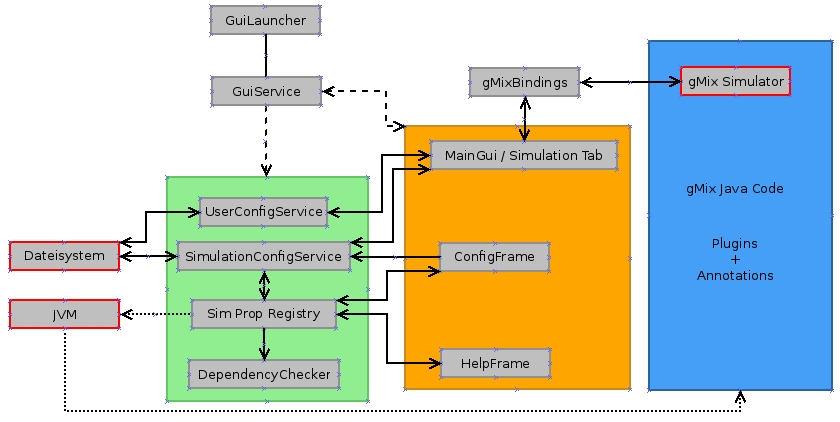
\includegraphics[width=\textwidth]{img/arch.png}
\caption{Aufrufhierarchie}
\label{fig:callgraph}
\end{figure}

Die GUI-Erweiterung für den gMix-Simulator besteht im Grunde aus zwei verschiedenen Arten von Komponenten. Zum einen gibt es die Dienste (grün hinterlegt) und andererseits gibt es die grafischen Elemente (orange hinterlegt). Die Dienste werden dabei von den grafischen Elementen verwendet um auf den Daten (z.B. SimProps) zu operieren. Somit sind Daten und Darstellung gemäß \emph{Model-View-Control Konzept} voneinander getrennt.\\

Der \emph{GuiLauncher} beinhaltet die \emph{main} Methode und stellt damit den Einstiegspunkt bei Starten der GUI dar. Der \emph{GuiLauncher} instanziiert als erstes die \emph{SimPropRegistry}, welche die Annotationen im Code des \emph{gMix} (blau hinterlegt) zur Laufzeit über die JVM ausließt. Anschließend wird ein initialer Check durch den \emph{DependencyChecker} durchgeführt. Im Anschluss wird die GUI aufgebaut, indem der \emph{GuiService} instantiiert wird. Dieser erstellt als erstes Instanzen von \emph{MainGui}, \emph{ConfigFrame} und \emph{HelpFrame}. Danach wird mittels des \emph{UserConfigService} die Benutzerkonfiguration geladen und die GUI wird so eingerichtet, wie der Benutzer sie verlassen hat. Nachdem dieses geschehen ist, greift die \emph{SimPropRegistry} über den \emph{SimulationConfigService} auf eine vordefiniertes EDF zu (etc/conf/experiment\_template.cfg) und ließt die Werte in die Properties ein. Bei jedem Einlesevorgang werden die relevanten GUI-Elemente neu gerendert. Im Anschluss führt der \emph{DependencyChecker} erneut eine Validierung auf allen Daten aus.

Nun ist die GUI komplett aufgebaut und eine gültige Konfiguration eingelesen. Der Benutzer kann nun mit der GUI (näheres in Abschnitt \ref{sub:guielemente}) interagieren. Die Arten der Interaktion können dabei grob in vier Kategorien unterteilt werden.

\begin{enumerate}
	\item Modifizieren der Konfiguration
	\item Verwenden der Hilfe
	\item Ausführung der Simulation und Evaluierung der Ergebnisse
	\item Beenden der GUI
\end{enumerate}

Das Verändern einer Konfiguration läuft wie folgt ab. Der Anwender sieht zu jedem Zeitpunkt die aktuelle Konfiguration im \emph{ConfigFrame} (auch \emph{Configuration View} genannt). Ändert der Benutzer dort einen Wert, so teilt das entsprechende GUI-Element dieses der \emph{SimPropRegistry} mit. Die Daten werden dann aktualisiert, der \emph{DependencyChecker} wird aufgerufen und anschließend werden die betroffenen GUI-Elemente aufgefordert ein Update durchzuführen.\\

Bei Laden und Speichern von Konfigurationen wird der \emph{SimulationConfigService} verwendet. Dieser wird entweder von dem \emph{SimulationTab} (auch \emph{Simulation View} oder dem \emph{ConfigFrame} aufgerufen. Beim Laden wird wie bei der Initialisierung ein vorhandenes EDF eingelesen und die Werte der SimProps werden dadurch überschrieben. Die Änderung des Wertes einer SimProp veranlasst wiederum das Updaten des entsprechenden GUI-Elementes und aktualisieren damit den \emph{ConfigFrame}. Beim Speichern hingegen ließt der \emph{SimulationConfigService} den aktuellen Zustand aller SimProps über die \emph{SimPropRegistry} aus und schreibt deren Werte in eine vom Benutzer festgelegte Datei auf dem Dateisystem.\\

Der \emph{HelpFrame} greift ebenfalls auf die \emph{SimPropRegistry} zu, um die vorhandenen Plugins auszulesen. Anhand dieser Information wird dann eine Menü aufgebaut, mit der der Anwender zwischen den HTML Seiten (je Plugin maximal eine HTML Seite) navigieren kann.\\

Wird eine Simulation gestartet, so teilt der \emph{SimulationTab} dem \emph{SimulationConfigService} den Pfad zu einer EDF mit. Diese wird eingelesen und als String an den \emph{SimulationTab} zurückgegeben. Anschließend wird das \emph{gMixBinding} aufgerufen, wobei der String mit den Informationen aus dem EDF als Parameter übergeben wird. Das \emph{gMixBinding} startet nun den \emph{gMix Simulator} als Thread. Sobald die Simulation beendet ist, teilt der \emph{gMix Simulator} dem \emph{gMixBinding} das Resultat mit, der Thread terminiert und das \emph{gMixBinding} gibt das Resultat an den \emph{SimulationTab} weiter, wo es dem Benutzer schließlich dargestellt wird.\\

Sobald der Anwender die GUI schließt, meldet sich die \emph{MainGui} bei dem \emph{UserConfigService}. Dieser fragt die GUI-Elemente nach Größe und Position (und einigen anderen Einstellungen) und speichert diese dann in einer benutzerdefinierten Konfigurationsdatei auf dem Dateisystem.

% subsubsection uebersicht (end)

\subsection{Wichtige Komponenten (Entwickler Informationen)} % (fold)
\label{ssub:einzelne_komponenten}
In diesem Unterabschnitt werden nun die wichtigsten Komponenten der \emph{gMix-Simulator-GUI} noch einmal ausführlich behandelt.

\subsubsection{SimPropRegistry}
\label{sssub:simpropregistry}
Die Klasse \emph{SimPropRegistry} ist die wohl wichtigste (und auch komplexeste) Hauptkomponente der gMix-Simulator-GUI. Ihre Aufgabe besteht darin, den gesamten Code des gMix-Simulators nach Annotationen abzusuchen und die in den Annotationen enthaltenen Informationen zu verarbeiten. Die \emph{SimPropRegistry} kennt dabei drei unterschiedliche Typen von Annotationen.

\begin{enumerate}
	\item Property Annotations (aka. SimProp)
	\item Plugin Annotations (aka. SimGuiPlugin)
	\item PluginSuperclass Annotations (aka. SimGuiPluginSuperclass)
\end{enumerate}

Die einzelnen Typen von Annotationen wurden bereits in Abschnitt \ref{sub:annotations} erläutert. Die \emph{SimPropRegistry} erzeugt anhand dieser Annotationen dann Plugin- und Property-Objekte, welche zur Laufzeit in verschiedenen Maps verwaltet werden. Neben den beiden wichtigsten Maps (\emph{properties} und \emph{plugins}), werden noch weitere Maps gehalten, welche beispielsweise die Menge der aktuell in der GUI ausgewählten Plugins halten (\emph{activePlugins}) oder aber andere zur Laufzeit wichtige Informationen speichern.\\

Des weiteren bietet die \emph{SimPropRegistry} einige Methoden an, um auf die Inhalte eben dieser Maps zuzugreifen. So beispielsweise eine Methode (\emph{setValue}), um Werte einer vorhandenen Property zu ändern. Die Plugin-Objekte hingegen sind komplett unveränderlich, da sie keine Informationen halten, die vom Benutzer editierbar sind. Es gibt allerdings die Methode (\emph{setActivePlugins}. Mit ihr kann die Auswahl der aktiven Plugins festgelegt werden. Die Information darüber welche Plugins aktiv sind, muss der \emph{SimPropRegistry} bekannt sein, da dieses beim Schreiben der EDF wichtig ist. Wir haben uns entschieden diese Informationen direkt in der \emph{SimPropRegistry} zu halten. Bei einer Zustandsänderung bezüglich der Konfiguration wird dann die \emph{SimPropRegistry} informiert und kann reagieren. Alternativ wäre es auch möglich gewesen, dass die \emph{SimPropRegistry} an kritischen Stellen das entsprechende GUI-Element nach seinem aktuellen Zustand fragt, dieses würde jedoch eine höhere Kopplung bedeuten, da die \emph{SimPropRegistry} dann die relevanten GUI-Elemente kennen müsste, weswegen wir diesen Weg vermieden haben.\\

Die \emph{SimPropRegistry} selbst ist als Singleton implementiert. Der Zugriff auf die \emph{SimPropRegistry} erfolgt über eine statische Methode (\emph{getInstance}) und kann an jeder Stelle im Code durchgeführt werden --- Diese Entscheidung wurde getroffen, da dieser Dienst in sehr vielen Komponenten der GUI verwendet wird und ein Durchreichen der Referenz in alle Komponenten sehr aufwändig und unübersichtlich wäre. 

\subsubsection{SimProp} % (fold)
\label{ssub:simprop}
Die Klasse \emph{SimProp} ist eine abstrakte Klasse und bildet die Oberklasse für die fünf typabhängigen Unterklassen (siehe Abb. \ref{fig:field_annotation}), die es zur Laufzeit geben kann. Die Felder der SimProp Unterklassen wurden bereits in Abschnitt \ref{sub:annotations} beschrieben. \\

\begin{figure}[!htp]
\begin{tikzpicture}
\umlsimpleclass[fill=blue!10]{SimProp}
\umlemptyclass[x=-3.5, y=-2, fill=blue!10]{BoolProp}
\umlemptyclass[x=-1.2, y=-2, fill=blue!10]{IntProp}
\umlemptyclass[x=1.2, y=-2, fill=blue!10]{FloatProp}
\umlemptyclass[x=3.9, y=-2, fill=blue!10]{DoubleProp}
\umlemptyclass[x=6.7, y=-2, fill=blue!10]{StringProp}
\umlVHVinherit[arm2=-1.2cm]{BoolProp}{SimProp}
\umlVHVinherit[arm2=-1.2cm]{IntProp}{SimProp}
\umlVHVinherit[arm2=-1.2cm]{FloatProp}{SimProp}
\umlVHVinherit[arm2=-1.2cm]{DoubleProp}{SimProp}
\umlVHVinherit[arm2=-1.2cm]{StringProp}{SimProp}
\end{tikzpicture}
\caption{Vererbung der Property Annotations}
\label{fig:field_annotation}
\end{figure}

 Obwohl alle Typen sehr viele Gemeinsamkeiten aufweisen, ist eine Typunterscheidung notwendig, da je nach Typ sich die Annotationen ein klein wenig unterscheiden (siehe \ref{ssub:feld_annotation}). So ergibt es beispielsweise keinen Sinn, einem \emph{Boolean} oder \emph{String} einen Minimal- oder Maximalwert zuweisen zu wollen, während dieses bei \emph{Integer}, \emph{Float} und \emph{Double} durchaus sinnvoll erscheint. Ein weiterer Vorteil ist, dass die Typkonversion und die Prüfung auf gültige Eingaben (sowie die Fehlerbehandlung) auch in die Unterklassen ausgelagert werden können, was der Lesbarkeit des Codes sehr dienlich ist. 

\subsubsection{UserConfigService} % (fold)
\label{ssub:userconfigservice}
Der UserConfigService verwaltet die \emph{user.properties}. In dieser Datei werden benutzerspezifische Einstellungen abgespeichert. Der Zugriff auf diese Datei ist nur aus dieser Klasse möglich. Beispiele für benutzerspezifische Einstellungen sind z.B. die Größe der einzelnen Fenster und ob sie separiert dargestellt werden sollen oder nicht.

\subsubsection{Requirement} % (fold)
\label{ssub:requirement}
Um die Abhängigkeiten zwischen verschiedenen Properties darzustellen, werden Requirements (Anforderungen) verwendet. Eine Anforderung wird dabei immer speziell für eine Property geschrieben. Um dem Entwickler maximale Freiheit zu gewähren kann die Abhängigkeit beliebig komplex gewählt werden.\\

Generell wird zwischen zwei Typen von Anforderungen unterschieden:
\begin{enumerate}
	\item Enable Requirements: Anforderungen die dazu führen das bestimmte Properties in Abhängigkeit zu anderen Property und deren Werten aktiviert oder deaktiviert werden.
	\\

	Ein Beispiel hierfür ist das "`Simulation Time End"' Requirement. Die Simulation kann entweder durch die Wahl "`Real Time"' beendet werden oder durch die Wahl von "`Simulation Time"'. Die beiden Optionen schließen sich somit gegenseitig aus. Daher ist es hier sinnvoll sie entsprechend zu deaktivieren/ aktivieren um den Benutzer zu unterstützen.
	\item Value Requirements: Anforderungen die dazu führen das bestimmte Properties in ihrem Wertebereich eingeschränkt werden. Dabei wurde die Implementation so gewählt, dass der vom Plugin Entwickler gewählte Wertebereich nicht erweitert werden kann weil dieses zu nicht sinnvollen Ergebnissen im Simulator führen würde.\\

	Ein Beispiel für ein Value Requirement ist die Einschränkung aufgrund von Minimal und Maximalwerten. Wenn eine Abhängigkeit zwischen diesen festgelegt wurde, gilt u.a., dass der aktuelle Maximalwert nicht kleiner sein darf als der aktuelle Minimalwert.
\end{enumerate}

\subsubsection{DependencyChecker}
\label{sssub:dependencychecker}
Der Dependency Checker dient der Überprüfung von verschiedenen Abhängigkeiten von einzelnen in den SimProperties definierten Anforderungen (Requirements).\\

Der Check findet bei jeder Änderung in der GUI statt. Im Fehlerfall, also wenn eine Anforderungen nicht eingehalten wird, gibt es zwei Fehlermechanismen:
\begin{enumerate}
	\item Enable Requirements: Die momentan nicht mögliche SimProp wird deaktiviert. Somit ist ein Auswählen / ändern nicht mehr möglich.

\begin{figure}[!htp]
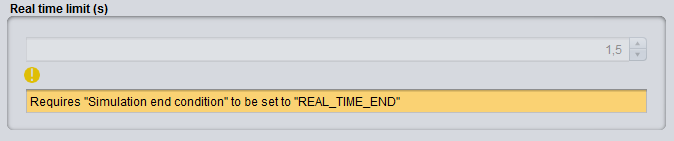
\includegraphics[width=\textwidth,scale=0.5]{img/DependencyChecker_RealTimeDisabled}
\caption{Deaktivierte Real Time End Property}
\label{fig:deactivatedRealTimeEnd}
\end{figure}

	\item Value Requirements: Falls neu gesetzte Werte aufgrund von Abhängigkeiten nicht mehr möglich sind, werden individuelle, in den Value Requirements definierte, Fehlermeldungen direkt in der Simpropery angezeigt.
	
	\begin{figure}[!htp]
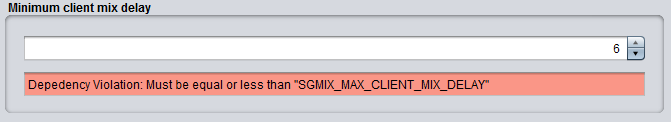
\includegraphics[width=\textwidth,scale=0.5]{img/DependencyChecker_MiniumClientMixDelayError}
\caption{Fehlermeldung bei Verstoß gegen Value Anforderungen}
\label{fig:errorMessageValueRequirement}
\end{figure}
\end{enumerate}

% subsubsection accordion (end)

\subsubsection{gMixBinding} % (fold)
\label{ssub:gmixbinding}
Die Klasse \emph{gMixBinding} ist eine Helfer-Klasse, die von der GUI verwendet wird, um den \emph{gMix-Simulator} mit der Konfiguration aus der GUI aufzurufen. Dazu war es notwendig, den Konstruktor des \emph{gMix-Simulators} so zu erweitern, dass er die Konfiguration als \emph{passthroughParameters} entgegennimmt. Der Aufruf des Simulators erfolgt als neuer Thread. Damit blockiert die GUI nicht, während die Simulation durchgeführt wird. Nachdem der Aufruf des \emph{gMix-Simulators} zurückkehrt, wird der Pfad zum Plot an eine Factory weitergereicht, welche ein GUI-Element erstellt, das für die Darstellung der Ergebnisse verantwortlich ist.\\

Ein bislang ungenutztes Feature, welches aber berücksichtigt wurde ist, dass in dem \emph{gMixBinding} das \emph{ResultSet} des Simulators bereitgestellt wird. Dieses beinhaltet die während der Simulation aufgezeichneten Statistik und kann dazu verwendet werden Ergebnisse anderweitig zu verarbeiten.\\

\section{Entwickler Anleitungen} % (fold)
\label{sec:entwicklung}
\subsection{DependencyChecker}
\label{ssub:dependencychecker}
Der Dependency Checker überprüft die Einhaltung von allen Value und Enable Requirements. Dies wird durch die Methode checkAll() realisiert, welcher die gesamte SimPropertyRegistry übergeben wird. Der Aufruf erfolgt dabei direkt nach dem Einlesen der Properties beim Start des Programms, wenn eine neue Konfiguration eingelesen wird, wenn für Plugins gescannt wird und immer wenn sich Daten in der SimPropertyRegistry ändern.
Die Funktion checkAll() arbeitet mit Reflections und versucht die übergebenen Enable und Value Anforderungen, die in der SimPropRegistry enthalten sind, zu instanziieren und auszuführen.\\

Dabei wird immer zuerst die Enable Anforderung überprüft, da wenn eine Property bereits deaktiviert ist, keine weitere Überprüfung auf valide Werte nötig ist.
\subsection{Requirement}
\label{ssub:Requirements}
Neue Anforderungen werden durch Erben von der abstrakten Requirement Klasse erzeugt. Ein neues Requirement muss somit immer die Methode check() implementieren, welche einen Boolean zurücklieferen muss. Da auf maximale Freiheit bei der Defintion der check() Methode gesetzt wurde, ist es auch möglich Werte beliebiger anderer SimProperty außer der eigenen SimProp zu ändern. Da dieses nur sehr schwer nachvollziehbar ist, ist es nach Konvention strikt verboten Werte anderer SimProps zu modifizieren.\\

Es existieren weiterhin in der abstrakten Requirements Klasse Hilfsfunktionen die bei der Erstellung von Requirements benutzt werden können.

\definecolor{sh_comment}{rgb}{0.12, 0.38, 0.18 }
\definecolor{sh_keyword}{rgb}{0.37, 0.08, 0.25}
\definecolor{sh_string}{rgb}{0.06, 0.10, 0.98}

\lstset{
	language=Java,
	basicstyle=\ttfamily\small,
	keywordstyle=\color{sh_keyword}\bfseries\small,
    stringstyle=\color{sh_string}\bfseries\small,
    commentstyle=\color{sh_comment}\itshape\small,
    frame=ltrb,
    breakindent=0pt,
    tabsize=2,
    lineskip=-0.3em,
	}
\begin{lstlisting}[caption={Beispiel: check() Methode einer Enable Anforderung}]
public boolean check() {
// getting the current SimPropRegistry
	SimPropRegistry gcr = SimPropRegistry.getInstance();
// getting the Simproperty at which this requirement 
// should be referenced
	SimProp simProp = gcr.getProperties().get(
		"REAL_TIME_LIMIT_IN_SEC");
//creating a warning message
	String msg = "Requires \"Simulation end condition\""+
	 	" to be set to \"REAL_TIME_END\"";
// create warnings if not existent
	if( simProp.getWarnings() == null ){
		simProp.setWarnings( new HashSet<String>() );
	}
// check property value on which the enable status 
// depends on, in this case the property "SIMULATION_END"
	if (equals("SIMULATION_END", "REAL_TIME_END")){
		//if it equals REAL_TIME_END we have to remove the 
		// warning which was eventually created before
		Set<String> warnings = simProp.getWarnings();
		warnings.remove(msg);
		simProp.setWarnings(warnings);
		// re-enable it
		simProp.setEnable(true);
		//return true because requirement is met
		return true;
		} else {
			// if there is another value we have to add 
			// the warning message to the warnings of 
			// the property
			Set<String> warnings = simProp.getWarnings();
			warnings.add(msg);
			simProp.setWarnings(warnings);
			// the requirement is not met so we have to 
			// disable the simprop and return false
			simProp.setEnable(false);
			return false;
		}
}
\end{lstlisting}
\subsubsection{Fehlermechanismus}
Um Fehler aus den Requirements in der GUI anzeigen zu lassen, empfiehlt sich die Nutzung der Errors oder Warnings der SimpProperties. Die Funktionen setErrors() und setWarnings() einer Property erwarten dabei ein Set<String> welcher die entsprechenden Meldungen beinhaltet. Sobald die Meldungen gesetzt sind werden sie automatisch angezeigt. 


\subsection{Erstellen eines neuen Plugins} % (fold)
\label{sub:neues_plugin}

Dieses soll ein Leitpfaden sein, der einem Pluginentwickler die Verwendung unseres Frameworks erleichtern soll. Wir gehen dabei davon aus, dass wir ein neues Plugin für einen existierenden Layer schreiben, da dieses der Regelfall sein wird.\\

Ziel ist es eine neue Implementation einer \emph{delayBox} zu entwickeln, die eine zufällige Verzögerung verursacht (ob dieses sinnvoll ist sei dahingestellt). Dazu wird als erstes die Datei \emph{RndDelayBox.java} unter \emph{src/evaluation/simulator/plugins/delayBox} angelegt. In diesem Verzeichnis befindet sich auch die Datei \emph{DelayBoxImpl.java}, welche die Definition der Oberklasse von DelayBoxen beinhaltet und die Schnittstellen festlegt. Der Quellcode dieser Klasse ist in Listing \ref{lst:dbox} dargestellt.

\begin{lstlisting}[caption={DelayBoxImpl.java}, label=lst:dbox]
...
@PluginSuperclass( layerName = "Underlay-net",
	layerKey = "TYPE_OF_DELAY_BOX", position = 7)
public abstract class DelayBoxImpl {

	public abstract int getSendDelay(
		int numberOfBytesToSend);
	
	public abstract int getReceiveDelay(
		int numberOfBytesToSend);
	
}
\end{lstlisting}

Die Klasse selbst ist schon mit einer \emph{PluginSuperclass} Annotation annotiert. Die Annotation legt fest, dass Plugins dieses Layers in der GUI unter der Kategorie \emph{Underlay - net} auftauchen, welche an Position 7 steht. Je höher die Position, desto weiter oben liegt der Layer in der \emph{Plugin Configuration} --- vlg. Abb. \ref{fig:guielements}. Der LayerKey ist ein eindeutiger String, der von der \emph{PluginRegistry} des gMix Simulators verwendet wird, um anhand der EDF das auswählte Plugin zu Bestimmen (Dieser String ist nicht frei wählbar, sondern wurde vom Entwickler des gMix Simulators so festgelegt).\\

Die neue Implementation soll eine zufällige Verzögerung mit oberer und unterer Schranke ziehen. Dafür benötigt das neue Plugin zwei Properties. Eine für das Minimum (vmin) und eine für das Maximum (vmax). Die fertige Implementation ist in Listing \ref{lst:rnddbox} dargestellt\\

\begin{lstlisting}[caption={RndDelayBox.java}, label=lst:rnddbox]
...
@Plugin(pluginKey = "RND_DELAY_BOX", 
	pluginName = "Random delay")
public class RndDelayBox extends DelayBoxImpl {
	
	@IntSimulationProperty(	name = "Minimum delay", 
			key = "RND_DELAY_BOX_MIN_DELAY", 
			property_to_vary = true, min = 0, max = 5)
	private int vmin = new Integer(
			Simulator.settings.getProperty(
					"RND_DELAY_BOX_MIN_DELAY"));
	
	@IntSimulationProperty(	name = "Maximum delay", 
			key = "RND_DELAY_BOX_MAX_DELAY",
			property_to_vary = true, min = 5, max = 10, 
			guiElement = "slider")
	private int vmax = new Integer(
			Simulator.settings.getProperty(
					"RND_DELAY_BOX_MAX_DELAY"));
	
	public RndDelayBox() {
		super();
	}
	
	@Override
	public int getReceiveDelay(int numberOfBytesToReceive) {
		return (int) (vmin + Math.random() * (vmax - vmin));
	}

	@Override
	public int getSendDelay(int numberOfBytesToSend) {
		return (int) (vmin + Math.random() * (vmax - vmin));
	}

}
\end{lstlisting}

Die neue Klasse erhält zuerst eine Plugin-Annotation. In der minimalen Konfiguration muss dort der \emph{pluginKey} für die Identifikation in der EDF und der \emph{pluginName} für die Darstellung in der GUI festgelegt werden. Der \emph{pluginKey} ist dabei eindeutig zu wählen und der \emph{pluginName} sollte nach Möglichkeit prägnant sein.\\

Die Properties müssen als Member der Klasse realisiert werden (die Initialisierung kann jedoch zu jedem beliebigen Zeitpunkt geschehen, also auch innerhalb von Funktionen). Diese Member erhalten nun abhängig von ihrem Typ die passende Property-Annotation. In diesem Fall handelt es sich um zwei \emph{IntSimulationProperties}. Property-Annotationen müssen immer einen \emph{key} und einen \emph{name} festlegen. Der \emph{key} identifiziert die Property in der EDF und der \emph{name} legt fest, wie die Property in der GUI auftritt. Soll eine Property variierbar sein, so muss dieses explizit durch \emph{property\_to\_vary = true} festgelegt werden. Bei numerischen Werten bietet es sich ebenfalls an den zulässigen Wertebereich durch \emph{min} und \emph{max} festzulegen. Es gibt bei Integern ebenfalls die Möglichkeit festzulegen, was für ein GUI-Element für die Benutzereingabe verwendet werden soll. Zu Demonstrationszwecken soll hier vmax mittels eines \emph{sliders} eingegeben werden (das Standardelement ist ein \emph{spinner}). \emph{vmax} und \emph{vmin} können nun in der Implementation verwendet werden.\\

Nun muss noch die Datei \emph{experiment\_template.cfg} angepasst werden, die die Standard EDF beinhaltet. Hier gilt es gültige Standardwerte für die beiden Properties festzulegen. Die Properties werden innerhalb der EDF durch ihre \emph{keys} identifiziert. Eine mögliche Anpassung ist in Listing \ref{lst:rnddboxedf} dargestellt.

\begin{lstlisting}[caption={Auszug aus der neuen experiment\_template.cfg}, label=lst:rnddboxedf]
...
TYPE_OF_DELAY_BOX = BASIC_DELAY_BOX
BASIC_DELAY_BOX_DEFAULT_CLIENT_BANDWIDTH_SEND = 131072
BASIC_DELAY_BOX_DEFAULT_CLIENT_BANDWIDTH_RECEIVE = 0
...
RND_DELAY_BOX_MIN_DELAY = 1
RND_DELAY_BOX_MAX_DELAY = 6
...
\end{lstlisting}

Zum Schluss muss noch die \emph{PluginRegistry} des gMix Simulators über das neue Plugin informiert werden. Dieses geschieht in diesem Fall in der Datei \emph{DelayBox.java}, welche im Verzeichnis \emph{src/evaluation/simulator/pluginRegistry} liegt. Dort muss das Enum um den \emph{pluginKey} des neuen Plugins erweitert werden. Des weiteren müssen die verschiedenen \emph{getInstance} Funktionen angepasst werden, so dass das neue Plugin verwendet wird, falls Simulator.settings.getProperty ("TYPE\_OF\_DELAY\_BOX") gleich ("RND\_DELAY\_BOX") ist.\\

Damit wäre das neue Plugin nun auch fertig und die GUI sähe im Anschluss wie in Abbildung \ref{fig:rnddbox} dargestellt aus. Auf die Verwendung von \emph{Requirements} wurde in diesem Leitpfaden verzichtet, da diese schon ausführlich im vorherigen Unterabschnitt behandelt wurden.

\begin{figure}[!htp]
\centering
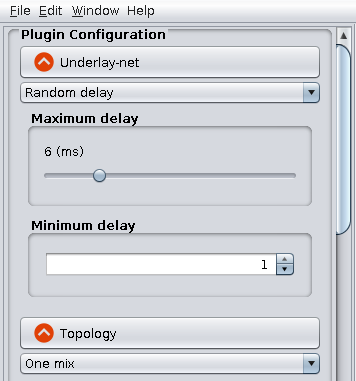
\includegraphics[scale=0.56]{img/rnddbox.png}
% subsection annotations (end)

\caption{GUI-Elemente für das neue Plugin}
\label{fig:rnddbox}
\end{figure}

Da an dieser Stelle nicht das komplette Framework abgedeckt werden kann, sei darauf hingewiesen, dass die bisher implementierten Plugins gute Beispiele darstellen, an denen man sich orientieren kann. Auch ein Blick in die Unterabschnitte \ref{ssub:feld_annotation} bis \ref{ssub:superclass_annotation} ist lohnenswert, da dort alle Felder der jeweiligen Annotationen erläutert werden.

% subsection erweiterung_von_simulation_property_annotationen (end)

%\section{Features} % (fold)
%\label{sec:features}
%Hier sollen später die Features unserer GUI aufgelistet und erklärt werden!

% TEST \cite{dummy:svs}.
% section features (end)

\newpage

\bibliographystyle{plain}
\bibliography{references}

%----------------------------------------------------------------------------------------

\end{document}